% CASE STUDY
\section{Case Study}
The study fundamentally adheres to the requirements for providing a publicly provisioned blockchain infrastructure that delivers security, privacy, and efficiency at an enterprise-grade level. The Logos Blockchain is designed specifically for certain use cases rather than being a general-purpose blockchain. However, the security model that will be implemented in the Logos chain, and presented in detail in this study, especially in section 4 (Findings), can possibly be applicable to other blockchain frameworks. The findings primarily present the core principles and methodologies that can be adapted to enhance the security and performance of blockchain systems generally, before presenting the possible substrate-based solution. 

In this section (case study), the general description of the case is first outlined, where a theoretical model of a blockchain is defined in its "default" form. This means that at this stage, we define the blockchain with a base architecture that is generally considered as secure. In Section 2.2 (Requirements), the general security requirements for an enterprise-grade blockchain infrastructure are presented. This leads to Section 2.3 (Specifications), where this requirements are clearly specified and defined to create a comprehensive picture of what an enterprise-grade security model demands in terms of security and privacy.

% DEFINITION
\subsection{Definition}
This research primarily focuses on the security and privacy aspects of a  blockchain network, it does not delve into aspects such as scalability, network performance, upgrade and maintenance capability, etc. These aspects will be addressed in a separate research project, focusing on achieving optimal efficiency in a distributed system like blockchain.

We first define here the "general security" in a blockchain network. For practical purposes, we designate it here as a \textit{general security model} and categorize it into four distinct sections. As elaborated in Chapter 1.2, this segmentation also streamlines the research of individual sections and the development of solution approaches independently, but they will must adhere to predefined fundamental network rules as they pertain to the entire system. Generally, we define the security aspect (general security model) of a blockchain network as follows.

\begin{enumerate}[label=(\arabic*)]
	% IDENTITIES, ACCESS CONTROL AND KEY MANAGEMENT 
	\item\textbf{Identities, Access Control and Key Management:}
	In blockchain systems, identity management, access controls, and key management are central security aspects. An \textit{identity} is represented by an \textit{account}, secured by a key pair consisting of a \textit{public and a private key}. The private key signs transactions, while the public key serves for identification within the network. Managing these keys includes secure creation, storage, and recovery.
	In addition to regular user accounts, there are also \textit{technical or service accounts} used for specific tasks or \textit{privileged operations}, such as smart contracts or oracles. These accounts often have special rights and access levels and are frequently protected by Hardware Security Modules (HSMs).
	A crucial concept is the use of \textit{session keys} (substrate term), which are temporary key pairs employed by validators. These keys are rotated regularly to enhance security and minimize the risk of long-term key compromises. Session keys enable validators to efficiently handle various critical tasks such as signing blocks and secure network communication. 
	\textit{Access controls} ensure that only authorized entities can access specific functions and data. Most modern frameworks typically offer the flexibility to implement customized \textit{role-based or attribute-based access control mechanisms}, although these mechanisms are not necessarily provided natively.

	% CRYPTOGRAPHIC MECHANISMS AND DATA PRIVACY
	\item\textbf{Cryptographic Mechanisms and Data Privacy:} 
	In blockchain systems generally, cryptographic mechanisms and data privacy are fundamental elements that ensure the security and confidentiality of data. Cryptographic algorithms such as \textit{SHA-256, Blake2b, and elliptic curve cryptography (ECC) (e.g., sr25519 and ed25519)} are utilized to ensure data integrity and authenticity. Hash functions like SHA-256 generate unique, immutable checksums for data, making any manipulation immediately detectable. ECC is used to create secure key pairs and digital signatures that authenticate transactions and protect against unauthorized modifications.
	In blockchains, these cryptographic mechanisms are closely tied to account management. As each \textit{account is secured by a key pair} consisting of a public and a private key. In addition to fundamental cryptographic mechanisms, there is increasing work on advanced techniques such as \textit{Zero-Knowledge Proofs (ZKPs)}. ZKPs allow the verification of the validity of information without revealing the information itself, significantly enhancing user privacy.
	\textit{Encryption} also plays a central role in \textit{data privacy}. Data stored on the blockchain can be protected using encryption techniques to ensure that only authorized parties have access to sensitive information. Various encryption methods can be applied to secure both data in "transit" and data at "rest".

	% CONSENSUS MECHANISMS AND NETWORK SECURITY
	\item\textbf{Consensus Mechanisms and Network Security:}
	In blockchain systems, consensus mechanisms and network security are crucial for ensuring the integrity and availability of the network. Consensus mechanisms determine how transactions are validated and new blocks are added to the blockchain. Frameworks typically support various consensus algorithms such as \textit{Proof of Stake (PoS), Proof of Authority (PoA), Practical Byzantine Fault Tolerance (PBFT)}, etc.
	There is also a specific variant of PoS called \textit{Nominated Proof of Stake (NPoS)}. NPoS is based on the principle that validators are elected by nominators who stake their tokens. This promotes decentralization and ensures that only trusted validators can create blocks. A critical security risk in blockchain systems is the \textit{51\% attack}. In a 51\% attack, a single entity or a coalition controls the majority of the network's hashrate (in Proof of Work) or staked tokens (in Proof of Stake). This allows them to manipulate transactions, perform double-spending, and censor or rewrite new blocks. This risk is mitigated by NPoS, where the selection and monitoring of validators are carried out by a broad community of nominators, making it difficult and costly to gain control over the network due to the involvement of multiple stakeholders.
	Proof of Authority (PoA), for example, relies on a limited number of trusted validators who are authorized based on their identity and reputation. While PoA enables high speed and efficiency, it is less relevant for public blockchains as it relies on trust in private parties. 
	In addition to consensus mechanisms, network security plays a central role. Network security measures include protection against \textit{Distributed Denial of Service (DDoS) attacks, Sybil attacks}, and other malicious activities. Networks implements mechanisms such as peer authentication, network segmentation, and the use of secure communication protocols like \textit{Transport Layer Security (TLS)} to ensure the integrity and confidentiality of data transmission.

	% AUDITING, POLICIES AND REGULATIONS
	\item\textbf{Auditing, Policies and Regulations:} 
    In blockchain systems, auditing, policies, and regulations are crucial components to ensure transparency, compliance, and trust. Auditing involves the systematic review and analysis of blockchain transactions and activities to detect and prevent fraud, ensure data integrity, and verify compliance with relevant standards and regulations.
	Blockchain frameworks, including Substrate, provide tools and mechanisms to facilitate comprehensive auditing. These include immutable ledgers that record every transaction, cryptographic proofs that ensure the integrity of data, and smart contracts that can automate compliance checks and reporting. Auditors can leverage these features to conduct real-time audits, trace transactions, and verify the authenticity of data on the blockchain.
	Policies define the rules and guidelines that govern the operation and use of the blockchain network. These policies may cover various aspects such as access control, data privacy, transaction processing, and security measures. Policies can be implemented and enforced through on-chain governance mechanisms, allowing stakeholders to propose, vote on, and enact changes to the network's rules and parameters.
	Regulations refer to the legal and regulatory frameworks that blockchain networks must comply with. These may include data protection laws, financial regulations, anti-money laundering (AML) requirements, and other legal standards. Compliance with regulations is crucial for ensuring the legitimacy and acceptance of blockchain technology in various industries. Substrate's modular architecture allows developers to build compliance into their blockchain applications, ensuring that they meet the necessary regulatory requirements.
	Effective auditing, robust policies, and strict regulatory compliance are vital for maintaining the integrity, security, and trustworthiness of blockchain systems. By leveraging the these principles its possible to implement comprehensive auditing practices, establish clear policies, and ensure adherence to relevant regulations, thereby fostering a secure and transparent blockchain environment.

\end{enumerate}

Implementing these security techniques is essential to ensuring the security, confidentiality, integrity, availability and authenticity od data, in a blockchain system.

% REQUIREMENTS
\subsection{Requirements}

% SPECIFICATIONS
\subsection{Specifications}

% FIGURE1
\begin{center}
	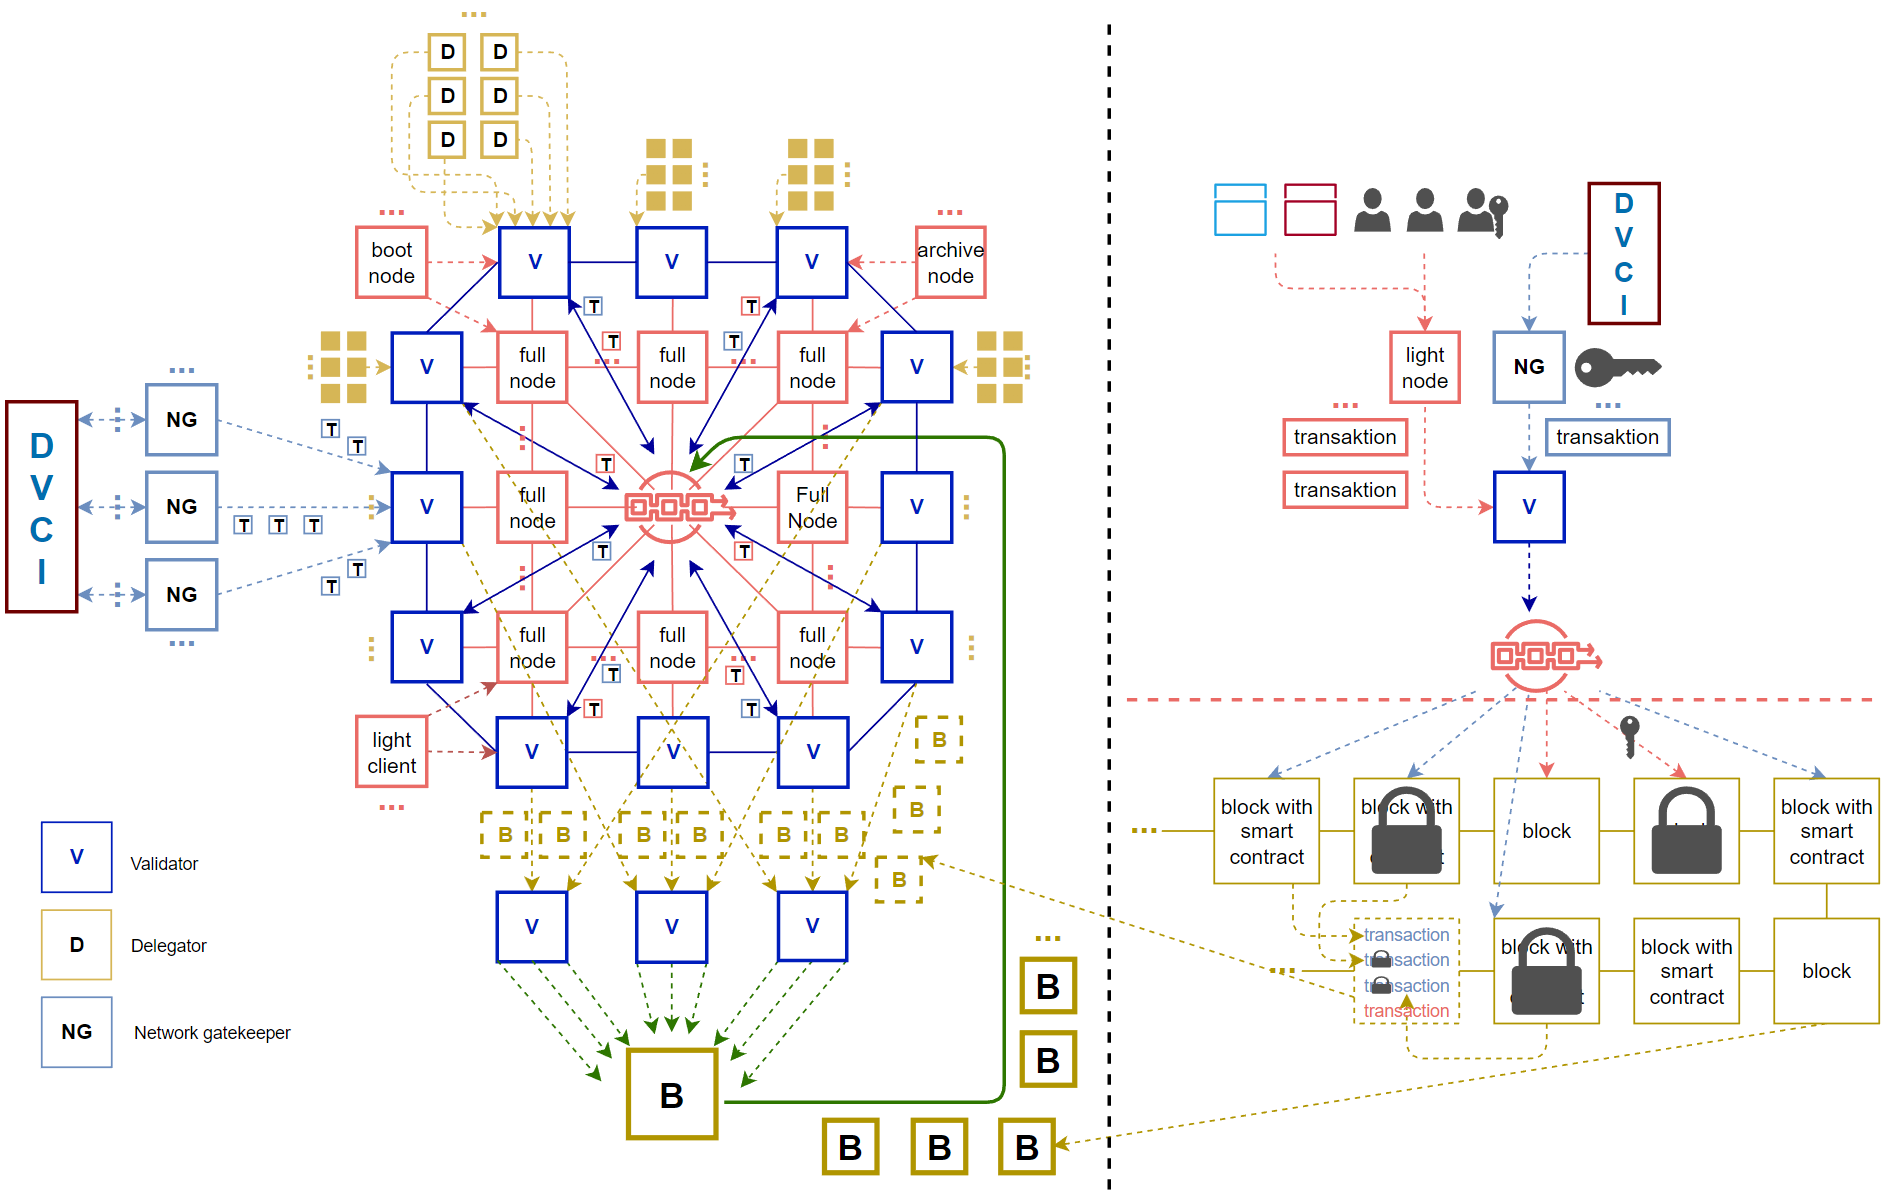
\includegraphics[height=10cm]{logos-chain}
\end{center}
\begin{center}
	Figure 1: 
\end{center}